\documentclass[fleqn,10pt]{wlscirep}
\usepackage[utf8]{inputenc}
\usepackage[T1]{fontenc}
\usepackage{listings}
\title{Preliminary Comparison of CRISPR/Cas9-based Screening Data Analysis Algorithms}

\author[1,*]{Y.Q. Yang}

\begin{abstract}
In the opening report of CRISPR/Cas9-based Screening Data Analysis, I introduced MAGeCK and BAGEL, which are both CRISPR/Cas9-based screening data analysis algorithms that can be applied for essential gene identification.  However, I only summarized the principles of two algorithms, but did not explicitly compare the difference between them in all aspects.  Therefore, I added detailed comparison information in this report, and preliminary process the screening data given by Professor Wang. Due to lack of time as well as corresponding data, the screening data were only calculated via MAGeCK.
\end{abstract}
\begin{document}

\flushbottom
\maketitle

\thispagestyle{empty}

\section*{Background}

MAGeCK and BAGEL are two known tools that have been specifically designed for CRISPR/CAS9-based essential gene identification. In order to find out which relatively performs better, I have to compare them from both their detailed algorithms in different steps and the actual analysis results obtained from on our own reserach data.  According to the above requirements, I generally planned my project workflow as below:

\begin{itemize}
    \item (1) Compare the principle of screening data analysis between two methods in all aspects(listed in order):
        \subitem read count calculation;
        \subitem read count normalization;
        \subitem sgRNA ranking;
        \subitem essential gene ranking;
    \item (2) Rank sgRNA and identify essential genes via two methods based on absolutely the same screening data.
    \item (3) Identify enriched pathway via MAGeCK only since this function is not inclued in BAGEL.
    \item (4) Compare MAGeCK with other pathway analysis tools and find out which one does a better job.
    \item (5) Summarize the tools that perform well at each step, improve the deficiencies, and thus generating a new workflow for CRISPR/Cas9-based essential gene and enriched pathway identification.
    \end{itemize}

\section*{Results}

\subsection*{Step-by-step Principle Comparison between MAGeCK and BAGEL}

\begin{table}[ht]
    \centering
    \begin{tabular}{lll}
    \hline
    Method & MAGeCK & BAGEL \\
    \hline
    read count calculation:\\
    $\quad$regard as "match probe" \\
    $\quad$when encounter single base mismatch & $\times$ & not mentioned \\
    \hline
    read count normalization & median normalization & not mentioned \\
    \hline
    sgRNA ranking:\\
    $\quad$basis of sgRNA abundancy testing \\
    $\quad$(between treatment and control)& p-value retrieved from NB model & log fold changes of frequency distribution\\
    \hline
    essential gene ranking:\\
    $\quad$algorithm & $\alpha$-RRA or MLS(in updated versions)& Bayes Factor\\
    $\quad$require reference geneset of training & $\times$ & \checkmark \\
    $\quad$require boundary values for scoring& $\times$ & \checkmark \\
    $\quad$have speed-up optimization& $\times$ & \checkmark \\
    \hline
    enriched pathway ranking & $\alpha$-RRA or MLS(in updated versions)& $\times$\\
    \hline
    \end{tabular}
    \caption{\label{tab:comparison}step-by-step principle comparison between MAGeCK and BAGEL}
    \end{table}

 
Detailed principle comparison between MAGeCK and BAGEL is listed in Table \ref{tab:comparison}.  It is clear that MAGeCK and BAGEL identify essential genes in totally distinct methods.  Although the developer of BAGEL claims that BAGEL has lower False Discovery Rate(FDR) rather than MAGeCK since the latter one ranks essential gene simply based on the experimental data and hence hard to prevent from unexpected data fluctuation; however, we still cannot rush to a final conclusion immediately without running these methods on our own data.
From my personal view, we should take on several experiments to test whether BAGEL can be reliable for our own-data analysis since we cannot find enough explanation about the details for each step.  First, we should test whether the essential-gene ranking results would change with the existence of different reference geneset.  Second, we should figure out its read count calculation and normalization methods to see what factors would affect the operating results.

\subsection*{Essential Genes identification based on our own reserach data}
In order to get familiar with the running workflow of these two methods and do preparation for later analysis, I analyzed the data given by Professor Wang via MAGeCK and got the analysis result, which was attached at the end of this report. 

In a regular workflow of MAGeCK operation, I have to prepare two groups of CRISPR/Cas9-based screening data.  One is the group treated with sgRNAs, and the other is the control group.  However, this time what I have got is two distinct groups with different sgRNA treatment.  One of which shows a upper concentration of cd69 proteins, while the other shows the opposite.  I doubt whether the data could be processed properly, so I asked Professor Wang for help.  He suggested that I could convert sample and control, and perform two sets of calculations respectively so as to reduce the error as much as possible. 

I calculated the read count in twice respectively as well, and retrieved two absolutely the same result in return.  This could tell us that the read count process is independent between different groups of data.

Contrary to the situation that happened in read count calculation step, completely different essential gene results are generated with $\alpha$-RRA scoring algorithm.  When regarding the cd69 higher expressed group as treatment group and lower expressed one as control, four genes are significantly essential: GRAP2, CCNL1, ZAP70, DOCK2.(see in Figure \ref{fig:up_down})  In contrast, three genes are regarded as essential in the converted analysis, that is: POFUT1, CTBP1, API5. (see in Figure \ref{fig:down_up}) 

Due to some limitation in the data I obtained, I decided to suspend the operation of BAGEL.  First, I am not sure whether BAGEL can perform properly under such groups of data.  Second, the genes I analyzed are immune-related, but the reference geneset provided by developers are cancer-related.  Considering that BAGEL is a supervised-machine learning like analysis method amoung which the selection of training data plays the key role in the method performance, I think is vital finding a much more proper reference geneset.


\section*{Discussion}
I have met some problems while running the program.

Noting that VISPR is a Visulization methods specialized for MAGeCK results that has been intergrated with MAGeCK recently, I decided to try running the entire process on the command "MAGeCK-VISPR" instead of the regularly used command "MAGeCK".  However, an unexpected error occurred in read count calculation step, showing that "command returned non-zero exit status 255".  I don't know the meaning of this error, nor could I find any similar case online as reference, so I have no chance but use the regular command "MAGeCK" instead, feeling sad not having experienced the visulizaiton function.

Even worse, I incorrectly estimated the data size as well as the time the program need for running.  I thought the program would run up to an hour;   however, when I realized the dramatically expensive computation cost, it was too late for me to make it up. In brief, there were 240496 predefined sgRNAs and 116315972 of total reads for the raw data of each case, which was far larger than I expected.  Furthermore, I meant to compare the differnce between $\alpha$-RRA and MLS, which are both essential gene ranking algorithm.  I found in the blog of MAGeCK previously that MLS performs better than $\alpha$-RRA in essential gene scoring, but it didn't mention that MLS is far more computationally expensive, which takes approximately an hour for simply one permutation.  Consequently, I fail to finish the MLE calculation, as well as the enriched pathway identification that I should have done. 




\begin{figure}[ht]
\centering
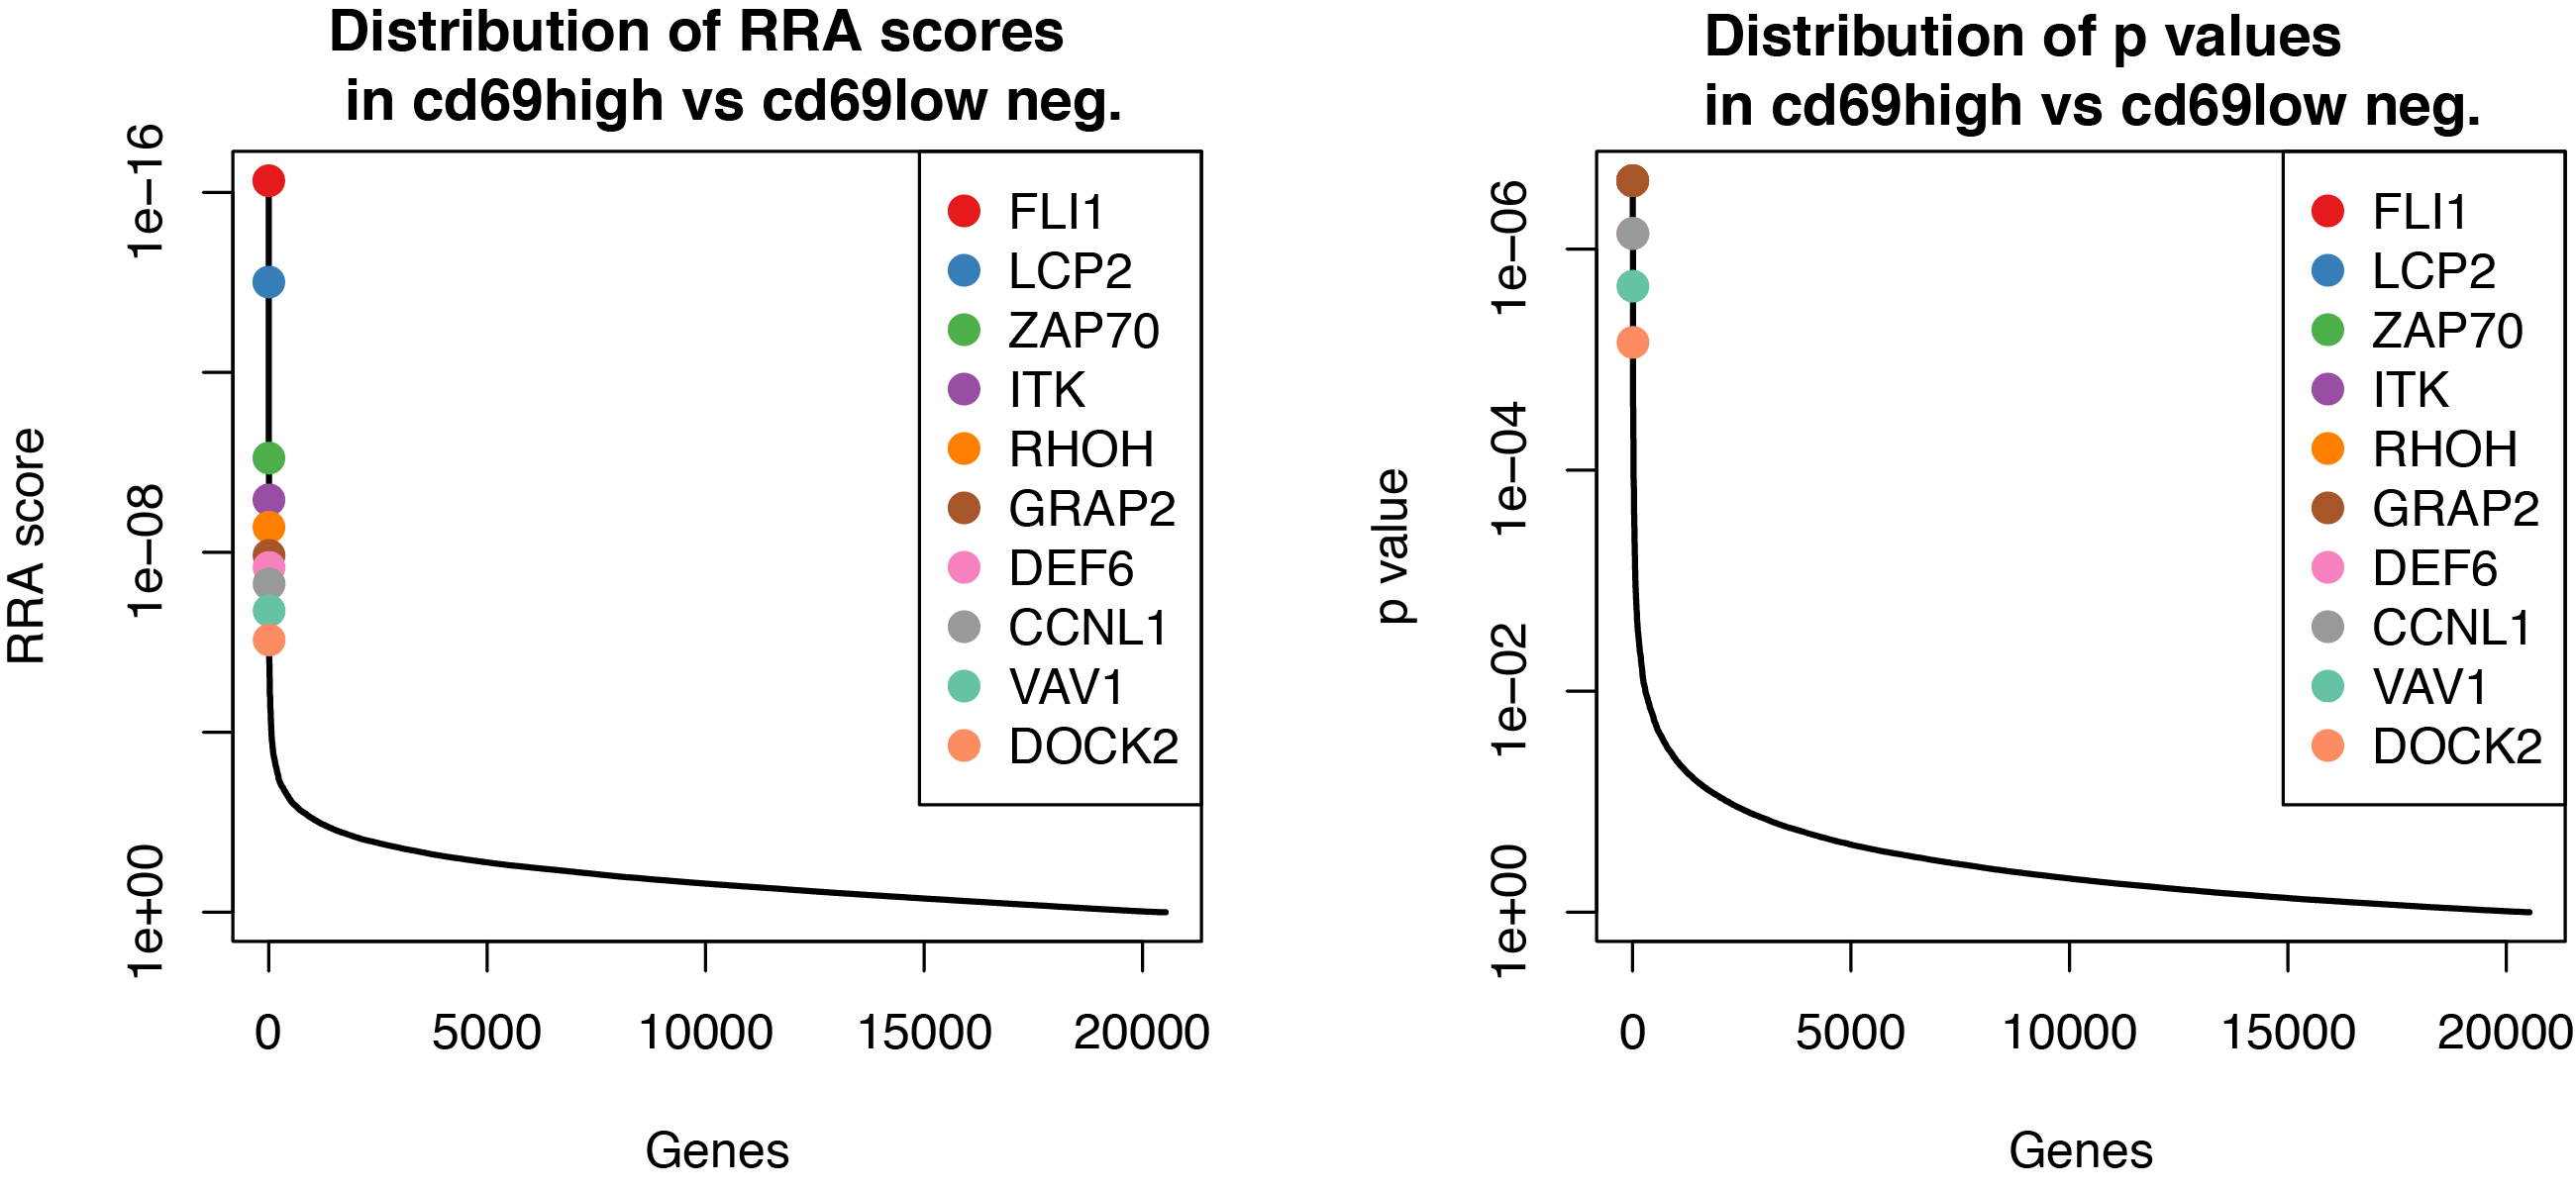
\includegraphics[width=\linewidth]{up_down}
\caption{Essential gene analysis result when regarding the cd69 higher expressed group as treatment group and lower expressed one as control.}
\label{fig:up_down}
\end{figure}

\begin{figure}[ht]
    \centering
    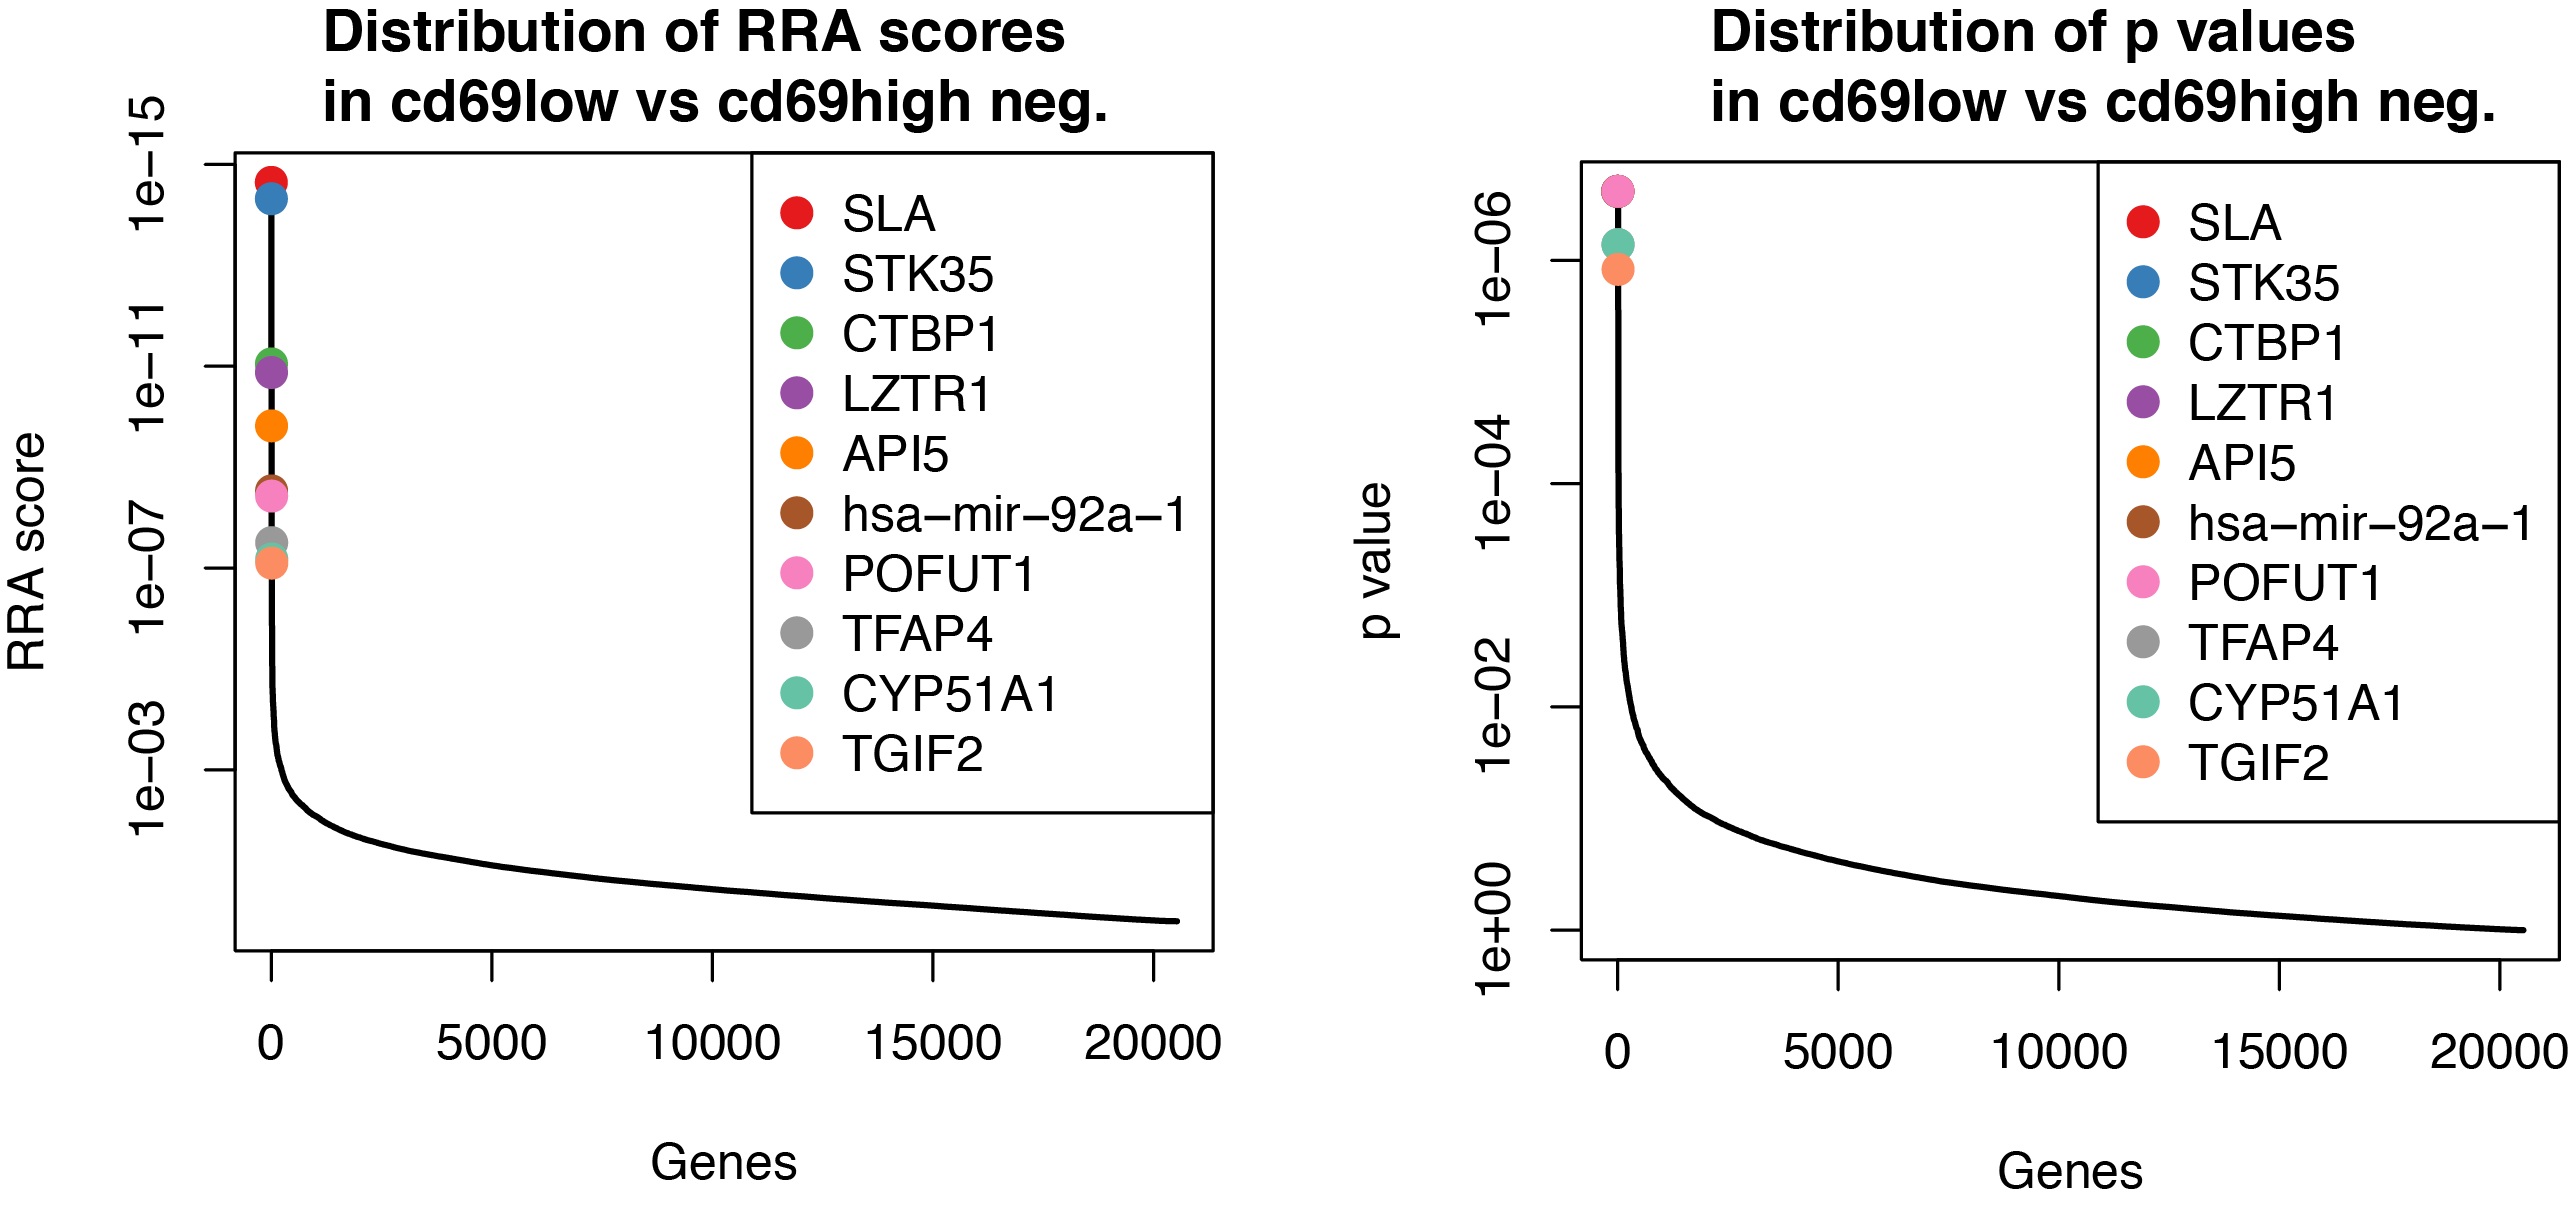
\includegraphics[width=\linewidth]{down_up}
    \caption{Essential gene analysis result when regarding the cd69 lower expressed group as treatment group and higher expressed one as control.}
    \label{fig:down_up}
    \end{figure}


\end{document}